\begin{frame}\frametitle{AUV Localisation using EKF in Practise}
\vspace{-5pt}
\begin{block}{}
\center{\textbf{There is no is no exact ground truth for underwater robot localisation available}}
\end{block} 
\centering
Issues to Address in AUV Localisation%\end{center}
\begin{columns}[t]
\column{.36\textwidth}
{\centering \textbf{Heading Measurement}} \\
{\centering \hspace{6pt} \includegraphics[width=0.25\linewidth]{fig/tcm.pdf} \hspace{15pt} vs.
\includegraphics[width=0.25\linewidth]{fig/kvh.pdf}} \\
	\begin{columns}[t]
	\column{.55\linewidth}
	{\centering	
	Compass {\footnotesize(\textit{yaw})} } \\
	\contra \begin{footnotesize}prone to noise\end{footnotesize} \\
	\contra \begin{footnotesize}calibration\end{footnotesize} \\
	\pro    \begin{footnotesize}absolute\end{footnotesize}  \\ %  meas.	
		
	\column{.44\linewidth}
	{\centering	
	Gyro \\ {\footnotesize(\textit{yaw rate})} \\
	\pro    \begin{footnotesize}accurate\end{footnotesize}	\\
	\contra \begin{footnotesize}relative\end{footnotesize}  \\
	} %  meas.
	\end{columns}
\vspace{10pt}
Apart from being ``fused'', measurements of \textit{yaw rate} and \textit{yaw} can be taken with adjustable confidence. 	
\column{.3\textwidth}
{\centering \textbf{Nonlinearity}} \\
UKF \cite{julier96} is an interesting alternative in handling nonlinearities. 
\includegraphics[width=0.85\linewidth]{fig/UKFpipeTrack.pdf} \\
\pro {\footnotesize model emulation} \\
\pro {\footnotesize computational cost}
\column{.31\textwidth} % on filtering those outliers. (absolute position)
{\centering \textbf{LBL imprecision}} \\ %LBL measurements exhibit quite diverse range of values. 
Position updates can deviate from the trajectory, resulting in outliers. EKF was compared with median filter.  \\  
{\centering
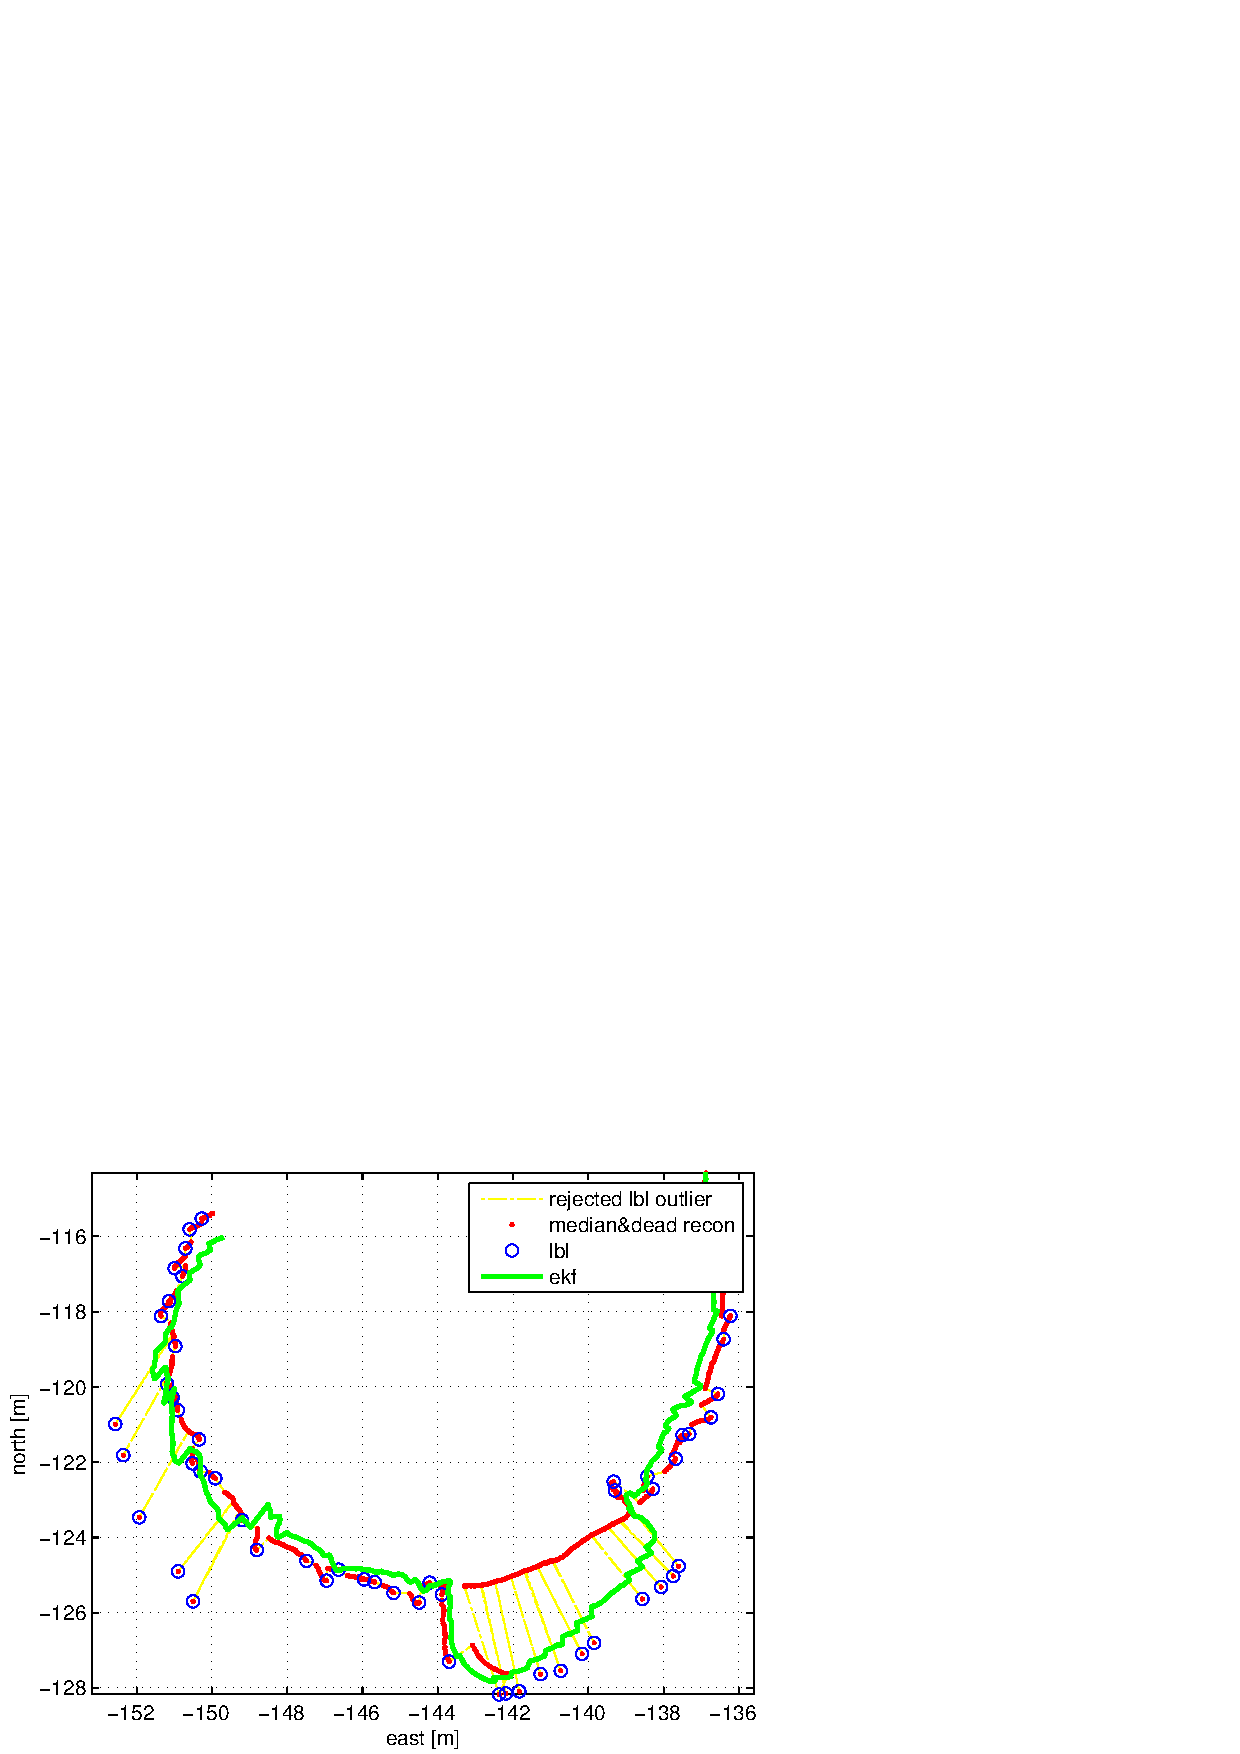
\includegraphics[width=0.8\linewidth]{fig/spiral-median-ekf.pdf} \\
\pro robust
} %outlier filtering 
\end{columns}
\end{frame}